\documentclass[landscape,final,a0paper,fontscale=0.285]{baposter}

\usepackage[vlined]{algorithm2e}
\usepackage{calc}
\usepackage{graphicx}
\usepackage{amsmath}
\usepackage{amssymb}
\usepackage{relsize}
\usepackage{multirow}
\usepackage{rotating}
\usepackage{bm}
\usepackage{url}
\usepackage{setspace}
\usepackage{wrapfig}

\usepackage{graphicx}
\usepackage{multicol}

%\usepackage{times}
%\usepackage{helvet}
%\usepackage{bookman}
\usepackage{palatino}

\newcommand{\captionfont}{\footnotesize}

\graphicspath{{images/}{../images/}}
\usetikzlibrary{calc}

\newcommand{\SET}[1]  {\ensuremath{\mathcal{#1}}}
\newcommand{\MAT}[1]  {\ensuremath{\boldsymbol{#1}}}
\newcommand{\VEC}[1]  {\ensuremath{\boldsymbol{#1}}}
\newcommand{\Video}{\SET{V}}
\newcommand{\video}{\VEC{f}}
\newcommand{\track}{x}
\newcommand{\Track}{\SET T}
\newcommand{\LMs}{\SET L}
\newcommand{\lm}{l}
\newcommand{\PosE}{\SET P}
\newcommand{\posE}{\VEC p}
\newcommand{\negE}{\VEC n}
\newcommand{\NegE}{\SET N}
\newcommand{\Occluded}{\SET O}
\newcommand{\occluded}{o}

%%%%%%%%%%%%%%%%%%%%%%%%%%%%%%%%%%%%%%%%%%%%%%%%%%%%%%%%%%%%%%%%%%%%%%%%%%%%%%%%
%%%% Some math symbols used in the text
%%%%%%%%%%%%%%%%%%%%%%%%%%%%%%%%%%%%%%%%%%%%%%%%%%%%%%%%%%%%%%%%%%%%%%%%%%%%%%%%

%%%%%%%%%%%%%%%%%%%%%%%%%%%%%%%%%%%%%%%%%%%%%%%%%%%%%%%%%%%%%%%%%%%%%%%%%%%%%%%%
% Multicol Settings
%%%%%%%%%%%%%%%%%%%%%%%%%%%%%%%%%%%%%%%%%%%%%%%%%%%%%%%%%%%%%%%%%%%%%%%%%%%%%%%%
\setlength{\columnsep}{1.5em}
\setlength{\columnseprule}{0mm}

%%%%%%%%%%%%%%%%%%%%%%%%%%%%%%%%%%%%%%%%%%%%%%%%%%%%%%%%%%%%%%%%%%%%%%%%%%%%%%%%
% Save space in lists. Use this after the opening of the list
%%%%%%%%%%%%%%%%%%%%%%%%%%%%%%%%%%%%%%%%%%%%%%%%%%%%%%%%%%%%%%%%%%%%%%%%%%%%%%%%
\newcommand{\compresslist}{%
\setlength{\itemsep}{1pt}%
\setlength{\parskip}{0pt}%
\setlength{\parsep}{0pt}%
}

%%%%%%%%%%%%%%%%%%%%%%%%%%%%%%%%%%%%%%%%%%%%%%%%%%%%%%%%%%%%%%%%%%%%%%%%%%%%%%
%%% Begin of Document
%%%%%%%%%%%%%%%%%%%%%%%%%%%%%%%%%%%%%%%%%%%%%%%%%%%%%%%%%%%%%%%%%%%%%%%%%%%%%%

\begin{document}

%%%%%%%%%%%%%%%%%%%%%%%%%%%%%%%%%%%%%%%%%%%%%%%%%%%%%%%%%%%%%%%%%%%%%%%%%%%%%%
%%% Here starts the poster
%%%---------------------------------------------------------------------------
%%% Format it to your taste with the options
%%%%%%%%%%%%%%%%%%%%%%%%%%%%%%%%%%%%%%%%%%%%%%%%%%%%%%%%%%%%%%%%%%%%%%%%%%%%%%
% Define some colors

%\definecolor{lightblue}{cmyk}{0.83,0.24,0,0.12}
\definecolor{lightblue}{rgb}{0.145,0.6666,1}

% Draw a video
\newlength{\FSZ}
\newcommand{\drawvideo}[3]{% [0 0.25 0.5 0.75 1 1.25 1.5]
   \noindent\pgfmathsetlength{\FSZ}{\linewidth/#2}
   \begin{tikzpicture}[outer sep=0pt,inner sep=0pt,x=\FSZ,y=\FSZ]
   \draw[color=lightblue!50!black] (0,0) node[outer sep=0pt,inner sep=0pt,text width=\linewidth,minimum height=0] (video) {\noindent#3};
   \path [fill=lightblue!50!black,line width=0pt] 
     (video.north west) rectangle ([yshift=\FSZ] video.north east) 
    \foreach \x in {1,2,...,#2} {
      {[rounded corners=0.6] ($(video.north west)+(-0.7,0.8)+(\x,0)$) rectangle +(0.4,-0.6)}
    }
;
   \path [fill=lightblue!50!black,line width=0pt] 
     ([yshift=-1\FSZ] video.south west) rectangle (video.south east) 
    \foreach \x in {1,2,...,#2} {
      {[rounded corners=0.6] ($(video.south west)+(-0.7,-0.2)+(\x,0)$) rectangle +(0.4,-0.6)}
    }
;
   \foreach \x in {1,...,#1} {
     \draw[color=lightblue!50!black] ([xshift=\x\linewidth/#1] video.north west) -- ([xshift=\x\linewidth/#1] video.south west);
   }
   \foreach \x in {0,#1} {
     \draw[color=lightblue!50!black] ([xshift=\x\linewidth/#1,yshift=1\FSZ] video.north west) -- ([xshift=\x\linewidth/#1,yshift=-1\FSZ] video.south west);
   }
   \end{tikzpicture}
}

\hyphenation{resolution occlusions}
%%
\begin{poster}%
  % Poster Options
  {
  % Show grid to help with alignment
  grid=false,
  % Column spacing
  colspacing=1em,
  % Color style
  bgColorOne=white,
  bgColorTwo=white,
  borderColor=red,
  headerColorOne=black,
  headerColorTwo=red,
  headerFontColor=white,
  boxColorOne=white,
  boxColorTwo=lightblue,
  % Format of textbox
  textborder=roundedleft,
  % Format of text header
  eyecatcher=true,
  headerborder=closed,
  headerheight=0.2\textheight,
%  textfont=\sc, An example of changing the text font
  headershape=roundedright,
  headershade=shadelr,
  headerfont=\Large\bf\textsc, %Sans Serif
  textfont={\setlength{\parindent}{1.5em}},
  boxshade=plain,
%  background=shade-tb,
  background=plain,
  linewidth=1pt
  }
  % Eye Catcher
  {
\includegraphics[width=16em]{images/mcgill_logo}} 
  % Title
  {\bf\textsc{\larger An Efficient Fault-Tolerant Sensor Fusion \\ \vspace{0.2em} Algorithm for Accelerometers}\vspace{0.3em} }
  % Authors
  {\textsc{O. Sarbishei, B. Nahill, A. Roshan Fekr, M. Janidarmian, K. Radecka, Z. Zilic \\
  {\smaller Department of Electrical \& Computer Engineering, McGill University, Montreal, Canada} \\
  B. Karajica \\
  {\smaller ST Microelectronics}
  }}
  % University logo
  {
\includegraphics[width=16em]{images/logo_iml_red}}

%\put(-15,545){
\includegraphics[width=0.7\paperwidth,height=13em]{images/bg_top.pdf}}
%\reflectbox{
%\put(-963,545){
\includegraphics[width=0.7\paperwidth,height=13em]{images/bg_top.pdf}}
%}

%%%%%%%%%%%%%%%%%%%%%%%%%%%%%%%%%%%%%%%%%%%%%%%%%%%%%%%%%%%%%%%%%%%%%%%%%%%%%%
%%% Now define the boxes that make up the poster
%%%---------------------------------------------------------------------------
%%% Each box has a name and can be placed absolutely or relatively.
%%% The only inconvenience is that you can only specify a relative position 
%%% towards an already declared box. So if you have a box attached to the 
%%% bottom, one to the top and a third one which should be in between, you 
%%% have to specify the top and bottom boxes before you specify the middle 
%%% box.
%%%%%%%%%%%%%%%%%%%%%%%%%%%%%%%%%%%%%%%%%%%%%%%%%%%%%%%%%%%%%%%%%%%%%%%%%%%%%%
    %
    % A coloured circle useful as a bullet with an adjustably strong filling
    \newcommand{\colouredcircle}{%
      \tikz{\useasboundingbox (-0.2em,-0.32em) rectangle(0.2em,0.32em); \draw[draw=black,fill=lightblue,line width=0.03em] (0,0) circle(0.18em);}}

%%%%%%%%%%%%%%%%%%%%%%%%%%%%%%%%%%%%%%%%%%%%%%%%%%%%%%%%%%%%%%%%%%%%%%%%%%%%%%
  \headerbox{Problem}{name=problem,column=0,row=0,span=1}{
%%%%%%%%%%%%%%%%%%%%%%%%%%%%%%%%%%%%%%%%%%%%%%%%%%%%%%%%%%%%%%%%%%%%%%%%%%%%%%
	Multi-sensor integration is growing in popularity due to greater availability of inexpensive sensor devices, providing new opportunities for greater accuracy and fault tolerance. For critical systems, fault response must be quick.
	
	We describe a new fault-tolerant MSE(Mean Square Error)-minimizing sensor fusion algorithm which can be used to improve sensor accuracy in multi-sensor systems while taking into account potential reliability issues of the sensors. Accelerometers have relatively high throughput for the low-power applications in which they are often encountered, necessitating a particularly efficient operation.
	
	The algorithm consists of three parts:
	\begin{enumerate}\compresslist
	\item Offline calibration
	\item Sensor fault screening
	\item Fusion of non-faulty sensor data
	\end{enumerate}
	\vspace{0em} % Space to align next box to the right
 }

%%%%%%%%%%%%%%%%%%%%%%%%%%%%%%%%%%%%%%%%%%%%%%%%%%%%%%%%%%%%%%%%%%%%%%%%%%%%%%
%  \headerbox{Contributions}{name=contributions,column=3,row=0}{
%%%%%%%%%%%%%%%%%%%%%%%%%%%%%%%%%%%%%%%%%%%%%%%%%%%%%%%%%%%%%%%%%%%%%%%%%%%%%%
%	\large \bf
%	To address the need for reliable sensor data from potentially faulty sensors in critical systems demanding quick fault detection and efficient fusion, we present the following:
%	\begin{enumerate}
%	\item A fault tolerant screening process to filter out faulty sensors
%	\item An MSE-minimizing linear fusion technique to operate on functional sensors
%	\item Test platforms for calibration and evaluation of accelerometers and temperature sensors
%	\end{enumerate}
% }

\headerbox{Fault Screening}{name=fault,column=3,row=0}{
\begin{algorithm}[H]
	\linesnumbered
	\dontprintsemicolon
	\SetKwComment{Comment}{// }{}
	\nl $x_{1:n}$ \Comment*[r]{\small $n$ sensor readings} \;
	\nl $M_{1:n}$ \Comment*[r]{\small Max deviation for sensor} \;
	\For{m in 1:n}{
		\nl $sum = \sum_{j=1}^{n}x_j$\;
		\nl
		\For{i in 1:n}{
			\nl $a_i=\frac{sum-x_i}{n-1}$\;
			\nl $d_i=\left| x_i - a_i \right|$\;
		}
		\For{i in 1:n}{
			\If{$d_i = \max{d_{1:n}}$}{
				\nl break\;
			}
			\If{$d_i > M_i$}{
				\nl Throw away $x_i$\;
				\nl $n = n - 1$\;
			}
		}
		\nl return $x_{1:n}$ \;
	}
\end{algorithm}
}

%%%%%%%%%%%%%%%%%%%%%%%%%%%%%%%%%%%%%%%%%%%%%%%%%%%%%%%%%%%%%%%%%%%%%%%%%%%%%%
\headerbox{Temperature Sensor Experimental Setup}{name=experimental,column=1,span=2,row=0}{
  %%%%%%%%%%%%%%%%%%%%%%%%%%%%%%%%%%%%%%%%%%%%%%%%%%%%%%%%%%%%%%%%%%%%%%%%%%%%%%

	\begin{multicols}{2}
\begin{wrapfigure}{r}[\columnwidth+\columnsep]{0.3\textwidth}
\begin{center}
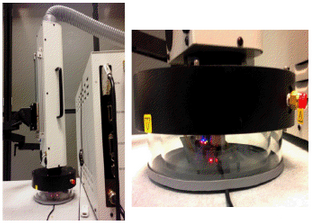
\includegraphics[width=0.3\textwidth]{tp4500}
\end{center}
\end{wrapfigure}
	
We developed a system of 8 STTS751 temperature sensors to log readings in a Temptronic TP4500 controlled temperature chamber for a reference.
	\end{multicols}
	\vspace{10em}
}
%%%%%%%%%%%%%%%%%%%%%%%%%%%%%%%%%%%%%%%%%%%%%%%%%%%%%%%%%%%%%%%%%%%%%%%%%%%%%%
  \headerbox{References}{name=references,column=0,above=bottom}{
%%%%%%%%%%%%%%%%%%%%%%%%%%%%%%%%%%%%%%%%%%%%%%%%%%%%%%%%%%%%%%%%%%%%%%%%%%%%%%
%    \smaller
%    \bibliographystyle{ieee}
%    \renewcommand{\section}[2]{\vskip 0.05em}
%      \begin{thebibliography}{1}\itemsep=-0.01em
%      \setlength{\baselineskip}{0.4em}
%      \bibitem{amberg11:graphtrack}
%        B.~Amberg, T. Vetter.
%        \newblock {GraphTrack}: {F}ast and {G}lobally {O}ptimal {T}racking in {V}ideos
%        \newblock In {\em CVPR '11}
%      \bibitem{awf:tracking}
%        A.~Buchanan and A.~Fitzgibbon.
%        \newblock {I}nteractive {F}eature {T}racking using {K-D} {T}rees and {D}ynamic {P}rogramming.
%        \newblock In {\em CVPR '06}
%      \end{thebibliography}
   \vspace{4em}
  }
%%%%%%%%%%%%%%%%%%%%%%%%%%%%%%%%%%%%%%%%%%%%%%%%%%%%%%%%%%%%%%%%%%%%%%%%%%%%%%
  \headerbox{Future Developments}{name=future,column=1,span=2,aligned=references,above=bottom}{
%%%%%%%%%%%%%%%%%%%%%%%%%%%%%%%%%%%%%%%%%%%%%%%%%%%%%%%%%%%%%%%%%%%%%%%%%%%%%%
  \begin{multicols}{2}
	%This method is very effective in the case that multiple sensors are expected to experience the same stimulus. This is particularly valuable for temperature sensors, gyroscopes on a rigid frame, and some fairly limited cases for accelerometers.
	
	%We would like to extend this work to cases where sensors 
  \end{multicols}
   \vspace{0.3em}
  }
%%%%%%%%%%%%%%%%%%%%%%%%%%%%%%%%%%%%%%%%%%%%%%%%%%%%%%%%%%%%%%%%%%%%%%%%%%%%%%
  %\headerbox{}{name=src,column=3,aligned=references,above=bottom}{
%%%%%%%%%%%%%%%%%%%%%%%%%%%%%%%%%%%%%%%%%%%%%%%%%%%%%%%%%%%%%%%%%%%%%%%%%%%%%%

  %}
%%%%%%%%%%%%%%%%%%%%%%%%%%%%%%%%%%%%%%%%%%%%%%%%%%%%%%%%%%%%%%%%%%%%%%%%%%%%%%
\headerbox{Accelerometer Experimental Setup}{name=speed,column=1,span=2,row=0,below=experimental,above=future}{
  %%%%%%%%%%%%%%%%%%%%%%%%%%%%%%%%%%%%%%%%%%%%%%%%%%%%%%%%%%%%%%%%%%%%%%%%%%%%%%
%\begin{tabular}{| c | c | c | c |}
%\end{tabular}
\begin{multicols}{2}

%\begin{wrapfigure}{l}{0.4\textwidth}
%\begin{center}
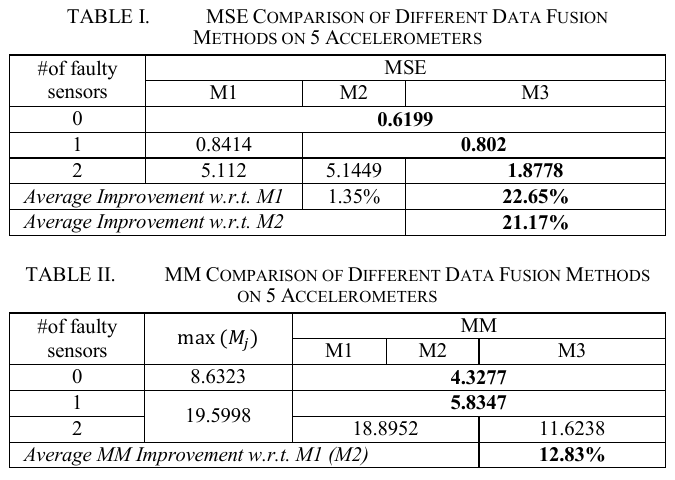
\includegraphics[width=0.4\textwidth]{result_tables}
%\end{center}
%\end{wrapfigure}

%\begin{wrapfigure}{r}{0.4\columnwidth}
%\begin{center}
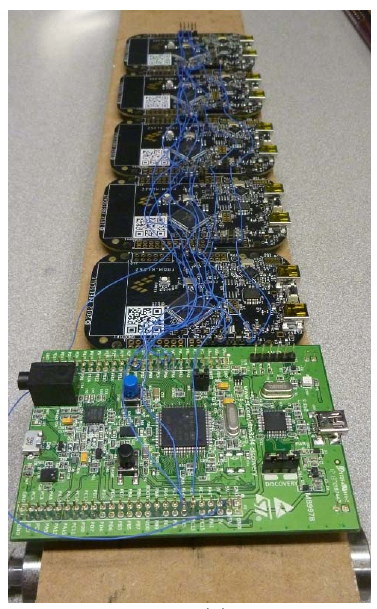
\includegraphics[width=0.25\textwidth]{acc_setup}
%\end{center}
%\end{wrapfigure}

\end{multicols}
}
%%%%%%%%%%%%%%%%%%%%%%%%%%%%%%%%%%%%%%%%%%%%%%%%%%%%%%%%%%%%%%%%%%%%%%%%%%%%%%
  \headerbox{Offline Calibration}{name=calibration,column=0,below=problem,above=references}{
%%%%%%%%%%%%%%%%%%%%%%%%%%%%%%%%%%%%%%%%%%%%%%%%%%%%%%%%%%%%%%%%%%%%%%%%%%%%%%
  %\noindent{\centering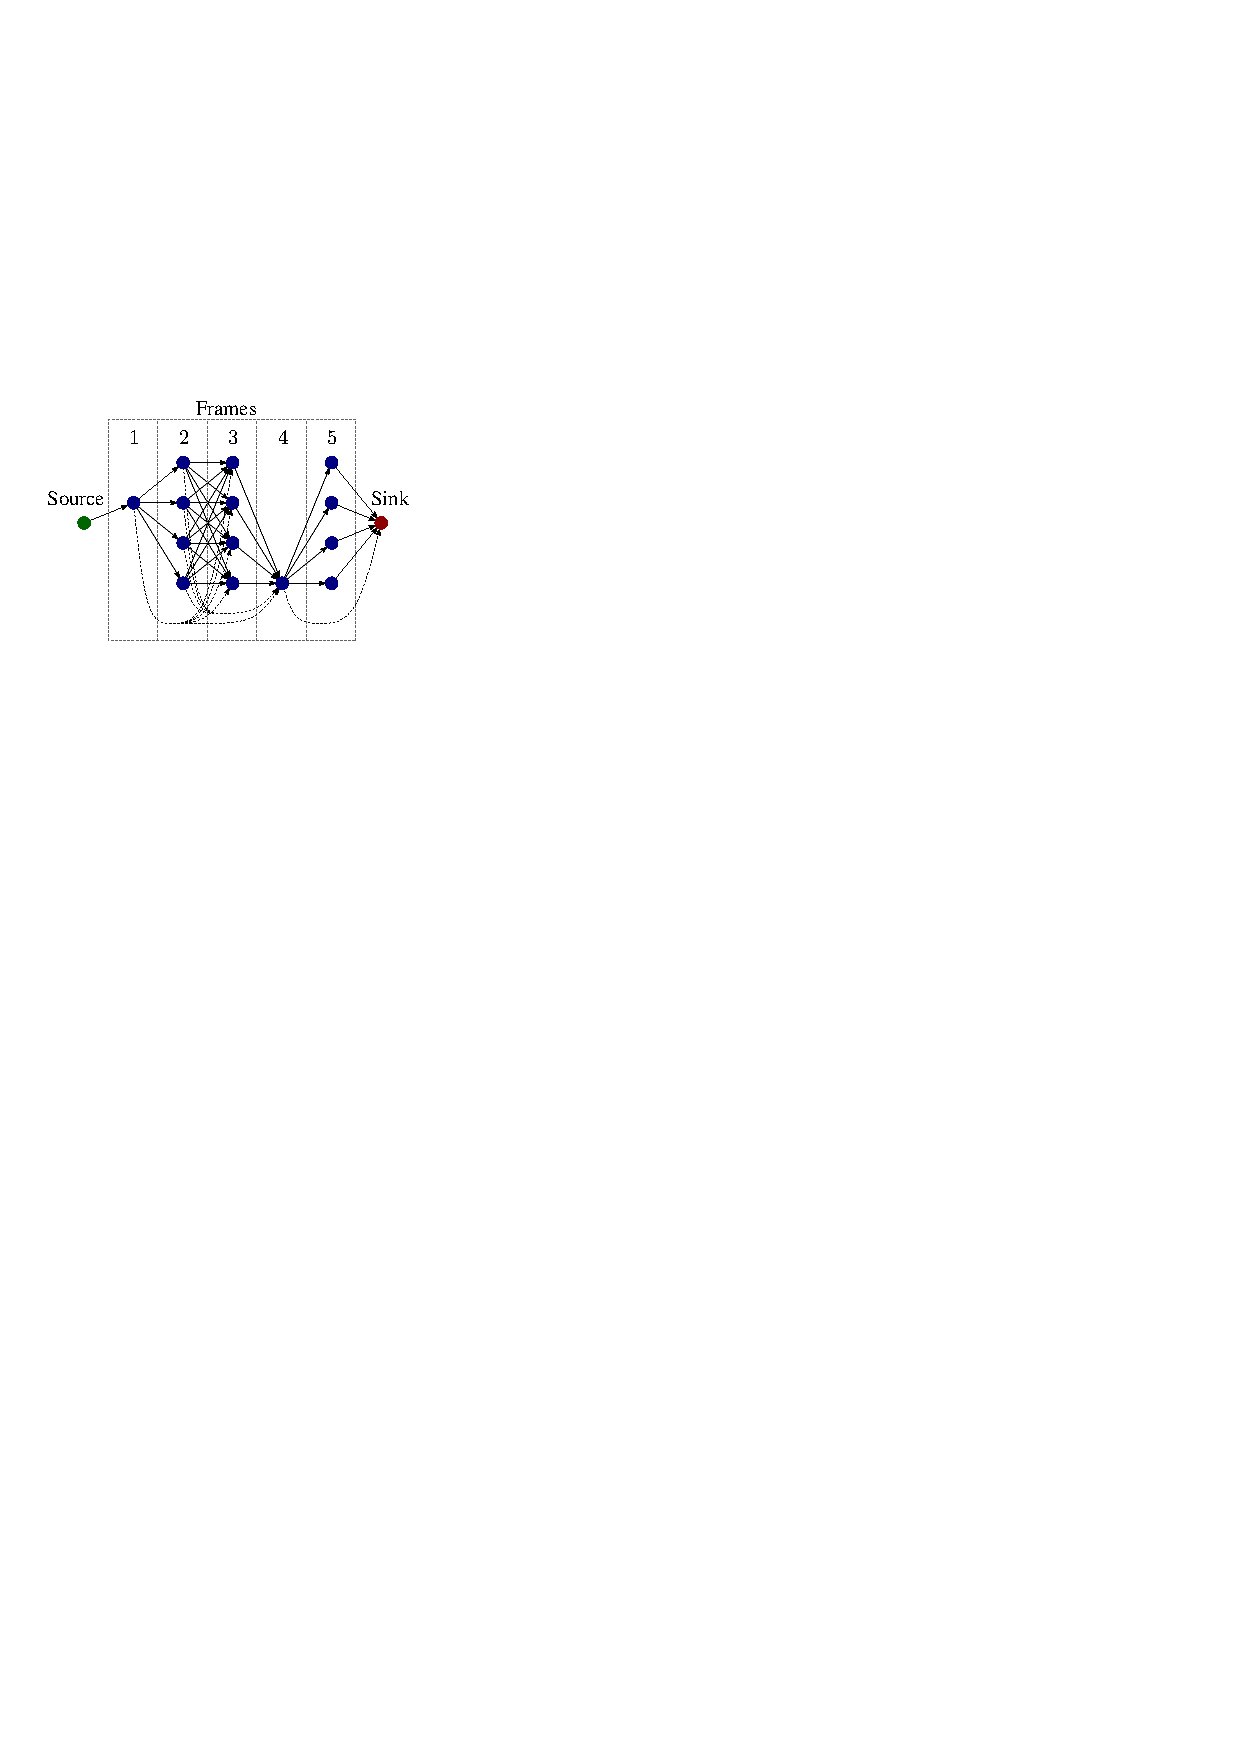
\includegraphics[width=0.95\linewidth]{images/graph_occluded.pdf}\\}
	An offline calibration is performed with all sensors mounted to account for discrepancies in manufacturing and mounting. Calibration is done with a collection of readings in 6 stationary positions. Coefficients are generated using the linear least-squares method (cite 24): \\
	Solve for calibration matrix $X$ in $Y = wX$ where $w$ are the raw sensor readings and $Y$ is the known reference vector, gravity. \\
	
	For our accelerometer experiments, over 30,000 values were considered.
  }
%%%%%%%%%%%%%%%%%%%%%%%%%%%%%%%%%%%%%%%%%%%%%%%%%%%%%%%%%%%%%%%%%%%%%%%%%%%%%%
  \headerbox{Accelerometer Fusion}{name=fusion,column=3,below=fault,bottomaligned=future}{
%%%%%%%%%%%%%%%%%%%%%%%%%%%%%%%%%%%%%%%%%%%%%%%%%%%%%%%%%%%%%%%%%%%%%%%%%%%%%%
\noindent Linear fusion: $\displaystyle x_{est}=\sum_{j=1}^{n}c_j x_j$ \\
\vspace{-0.3em}
For an error function independent of $x_{ref}$, \\
\vspace{-0.5em}
\begin{align*}
x_{ref}(1-\sum_{j=1}^{n}c_j)=0 \Longrightarrow \sum_{j=1}^{n}c_j = 1
\end{align*}
\vspace{-0.8em}
Optimal coefficients are \\
\vspace{-0.8em}
\begin{align*}
c_j = \frac{1}{S_j \sum_{k=1}^{n}\frac{1}{S_k}}
\end{align*}

where $S_j$ is the average square error for sensor $j$. For zero-mean error (proper calibration), this is the noise variance.
}

\end{poster}

\end{document}
